\documentclass{article}
\usepackage{amsmath}
\usepackage{amssymb}
\usepackage{graphicx}
\usepackage{soul}
\usepackage{anysize} %<-for setting margins
\marginsize {1.6cm}{1.6cm}{2.0cm}{2cm}
\usepackage{color}
\newcommand{\dean}[1]{\textcolor{red}{#1}}
\newcommand{\mike}[1]{\textcolor{green}{#1}}
\newcommand{\parham}[1]{\textcolor{blue}{#1}}

\title{Responses - Spatiotemporal Multi-Resolution Approximation of the Amari Type Neural Field Model}
\author{ P. Aram, D. Freestone, M. Dewar, K. Scerri, V. Jirsa, D. Grayden, V. Kadirkamanathan}

\begin{document}
    \maketitle

    The authors would very much like to thank the reviewers for their encouraging comments and their efforts to help improve this paper. Please find below the authors responses to the reviewers questions and suggestions regarding the manuscript. 
\\

Best Regards,
\\

Parham Aram.

\section{Handling editor}
\begin{enumerate}
\item Whilst the paper does fit the scope of NI, I agree with R1 and R3, that explicit advantages of going to a multiresolution frame - in addition to the conceptual ones - compared to the prior work based on Gaussian basis functions needs clarification and elucidation. 

\emph{Response here.}

\item  In addition, at least a `proof of principle" inversion from empirical data would enhance the potential impact of the paper. 

\emph{Response here.}
	
\end{enumerate}

    \section{Reviewer 1}
    
    % It would be useful to mention the above (now below) explicitly in the introduction and try to address them in later sections of the paper.

    \begin{enumerate}
        \item The exposition of the material and the relevant discussion have many similarities with the papers of the same authors (Freestone et al., 2011) and (Dewar et al., 2009) published in Neuroimage and IEEE Trans on Signal Processing  respectively.

	\emph{Response here.}
	
        \item The authors say the paper at hand is an ``extension'' of Freestone et al. by which I understand they mean the use of a wavelet as opposed to a Gaussian basis for the decomposition.

	\emph{Response here.}

        \item Since the methodology used is the same as in that earlier Neuroimage paper, the paper at hand repeats several of  the results of that previous paper, see sections 3 and 4: equations (2)-(5) and (20) -(33) have already appeared or are very similar to equations in Freestone et al.

	\emph{Response here.}
	        
        \item Section 5 is a review of known results and standard background material from wavelet theory and includes a simple calculation of the Fourier transform of the particular basis used here, which would be more appropriate for an appendix (cf appendix H of the Freestone et al. paper where the Fourier transform of the Gaussian basis functions is calculated).

		\emph{Response here.}

        \item Section 6 also borrows heavily from Dewar et al, e.g. cf equation (58) of this paper with equation (19) of Dewar et al: the state transition matrix is a perturbation of the corresponding matrix used in that earlier paper. The approach used in both papers seems to be the same with an RTS smoother used in the E-step (this was also used and explained in Freestone et al.) and an M step optimizing a cost function, quadratic in the parameters, cf. equation (62) with  equation (29) of Theorem 2 of Dewar et al. In general, the derivations of section 6 and appendix B follow closely or are very similar to those of Dewar et al.

		\emph{As the reviewer correctly pointed out there are similarities in the derivations herein and that of Dewar et al. Our main aim here is to adapt techniques from control systems theory and machine learning, modify and apply them to the Amari type neural field models. As the result some of the derivations are naturally similar. For example, the Amari type neural field model in this paper is only different to the IDE model in Dewar et al. due to the membrane time constant and the firing rate, as the result the only changes appear in the transition matrix is the presence of the membrane parameter $\xi=1-T_s/\tau$ and the firing rate slope $\varsigma$. The use of the RTS smoother in the E-step of the EM algorithm for state space models is an effective, standard and widely used approach. In fact, the aim of the IDE representation in a state space form is to adapt the EM and consequently the RTS smoother. The RTS algorithm is presented only for completeness and it is different than Unscented RTS (for non-linear state space models) in Freestone et al. The cost function of the linear state space model is always quadratic in parameters in the M-step ??? in fact it is one of the advantages of this representation giving a closed form solution for system's parameters.  The novel implementation of the M-step in this work significantly simplifies the computational complexity of the EM based algorithm proposed by Dewar et al. as it is shown in Table.~4 of the manuscript, namely from $O(n_x^4n_{\theta}^2)$ to $O(n_x^2n_{\theta}^2)$. This reduction is very significant and crucial for high dimensional systems and specifically for implementing the multi-resolution framework introduced here which otherwise would be possible. }
		
        \item Also, Appendix A is the analogue of Appendix D of Freestone et al. and Appendix C includes results known from the literature (as the authors point out).

\emph{Response here.}

        \item Although I value the use of a wavelet as opposed to a Gaussian basis, the advantages in the context of the analysis of brain imaging data have not been demonstrated and a comparison with the authors' earlier approach has not been performed.  The framework of Freestone et al., seemed not to assume a linear relation between mean membrane potential and firing rate and in that sense the present approach appears more restrictive.

\emph{Response here.}

        \item The authors say that a multi-resolution approach would explain the``organizational level of the brain at which cognition and behaviour are best explained'' but it is unclear what the alternative levels considered here are and what the significance of the results obtained is.

\emph{Response here.}

				\item Similar claims to the ones mentioned here regarding  implications for ``patient-specific'' modelling have also been made in Freestone et al., so it is not clear how these relate to the current multi-resolution approach and also such remarks might look too ambitious given that only synthetic data with fixed parameters are considered.
				
				\emph{Response here.}
				
				\item The comments about model complexity and parsimony on p.13 are somehow vague as these quantities are undefined.
				
				\emph{Response here.}
				
				\item Also, the comments on large scale networks and delays made on p.20 look irrelevant to the present framework.
				
				\emph{Response here.}
				
				\item Much of the discussion of the last section focuses on technical issues, while the discussion of the observation kernel chosen on p.17 is limited.
				
				\emph{Response here.}

    \end{enumerate}
    
    \section{Reviewer 2}
    
\begin{enumerate}
    \item As a minor comment, I would suggest changing the notation for the scaling and wavelet coefficients in Eq. (6), for example into normal lowercase `a' and `c', respectively. The $\beta$ might be confused by B-spline notation. 

	\emph{Response here.}

\item For the discussion, it might be useful to add a sentence that the basis structure (i.e., non-redundant, versus a (tight) frame representation) is a requirement for this framework.

\emph{Response here.}



\item A small comment might also be considered for Sect 8.2: it is possible to apply other than dyadic subsampling schemes in multiple dimensions, which leads to less wavelet subbands. For example, in 2D, the quincunx scheme is well-known to have better isotropic properties. Unfortunately, in 3D, it is not possible to have a subsampling operator (acting on a Cartesian sampling lattice) that is performing subsampling at equal rate in each dimension at each iteration, see Van De Ville et al,`On the multidimensional extension of the quincunx subsampling lattice', IEEE SPL, 12:2, pp.  112-115, 2005, for a comment on this. 

\emph{Response here.}


 % 
 % \begin{figure*}[!ht]
 % \begin{center}
 % 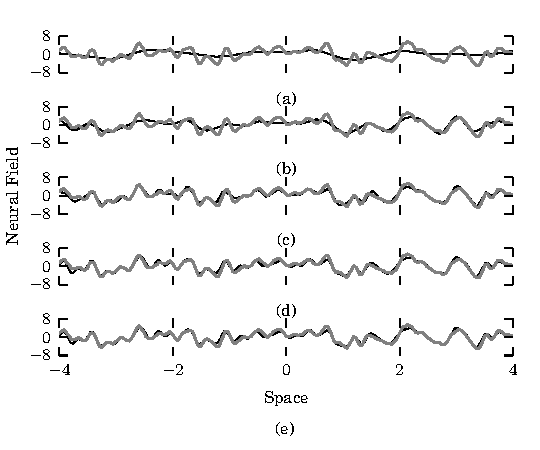
\includegraphics{./Graph/pdf/fig1.pdf} 
 % \end{center}
 % \caption{}
 % \label{fig:Figure1}
 % \end{figure*}

 

\end{enumerate}  

    \section{Reviewer 3}  
    \subsection{Main Concerns}
		\begin{enumerate} 
			\item I am not at all sure that isotopic scaling of the multiresolution is appropriate for brain connections, but I cannot say at this point that it is not.
			
			\emph{Response here.}
			 
			\item This model cries out for validation in real neuronal systems, but alas, at this point we only see convergence to synthetic data.   
			
			\emph{The authors appreciate that the only way to truly validate the proposed framework is with real data. However, before validating the method on real data we believe that it is essential to first validate the estimation method using accepted models and synthetic data, where the true and estimated parameters can be compared. In an effort to make the method employed in the paper more explicit, we have added ``To illustrate the estimation framework, data is generated using the neural field equations incorporating modeled sensors enabling a comparison between the estimated and true parameters'' to the introduction. We plan to validate the framework on real data in future work. We have added that validating the framework on real data is required in the Conclusion.}  
			
			\item This audience needs to have all symbols, including commonly used ones such as `equality over distribution', double font domains like R and Z, and jargon terms such as `lead field'.
			
			\emph{Response here.}  
			
			\item I would off-load all of the very difficult mathematics to the appendices and supplementary data, and focus a NeuroImage paper on the results of image analysis. 
			
			\emph{Response here.}
			
			\item Contrasting, for example, this multiresolution method with Freestone's 2011 results would be helpful for continuity.
			
			\emph{Response here.}
			
			\item I would also recommend archiving code that, for instance generates figure 11, so that the readership has a chance to replicate these findings, and adapt this method to their own data.
			
 			\emph{Response here.}
 		
			                                       
			\end{enumerate}  
			\subsection{Moderate concerns} 
			\begin{enumerate} 
			 \item Page 2: the authors should clearly define the difference between neural field and neural mass models.
			
			\emph{Response here.}
			
			\item Eqn 3: theta needs indexing 
 
			\emph{Response here.}
 			
			\item Define first and second order synaptic responses (used in figure 2 to explain text that does not refer to these terms)
			
			\emph{Response here.}
			
			\item{Eqn 9: the state variables $x$ seem to arise without distinction from $v$}  
			
			\emph{Response here.}
			
			\item Between eqn 19 and 20 change
			`write the neural field and connectivity kernel decomposition' To `write the connectivity kernel and neural field decomposition'
			To maintain order with eqns 20 and 21.

			\emph{Response here.}
			
			 
			 \end{enumerate}  
			\subsection{Trivia}
			\begin{enumerate}
			 \item 	Define `one-off' on pg 16 

 			\emph{Response here.}

  		\item Figure 8 is referred to in the text out of order

  			\emph{Response here.}
			 
			\item Pg 19: `stationary point i.e. global' should be `stationary point, i.e. a global'

			\emph{Response here.}			
			                   
			
			 
				\end{enumerate} 
				
			
\end{document}